\newcommand{\dropperTagResultsAucTable}{
    \begin{table}[H]
        \centering
        \begin{tabular}{|p{2,8cm}||P{2,4cm} P{2,4cm} P{2,4cm}|}
            \hline
            Dropper Tag & ALOHA\newline (M/B only) & ALOHA & Proposed\newline Model \\
            \hline
            AUC-ROC & - & 0.547$\pm$0.077 & \textBF{0.550$\pm$0.027} \\
            \hline
        \end{tabular}
        \caption[Dropper Tag prediction task AUC-ROC results]{AUC-ROC (Area Under Curve) of the different models for the \textbf{Dropper Tag} prediction task. Results were aggregated over \textBF{2} training runs with different weight initializations and minibatch orderings. Best results are shown in \textbf{bold}.} \label{tab:dropperTag_auc}
    \end{table}
}

\newcommand{\dropperTagResultsAtFprTable}{
    \begin{center}
        \begin{longtable}[c]{|P{3,2cm}||P{1,8cm} P{1,8cm} P{1,8cm} P{1,8cm} P{1,8cm}|}
            \hline
            Dropper Tag & \multicolumn{5}{c|}{{FPR}} \\
            & $10^{-5}$ & $10^{-4}$ & $10^{-3}$ & $10^{-2}$ & $10^{-1}$ \\
            \hline
            \endfirsthead

            \caption*{\raggedright ...continued from previous page} \\
            \hline
            Dropper Tag & \multicolumn{5}{c|}{\textbf{FPR}} \\
            & $10^{-5}$ & $10^{-4}$ & $10^{-3}$ & $10^{-2}$ & $10^{-1}$ \\
            \hline
            \endhead

            \caption*{\raggedleft ...continued on next page} \\
            \endfoot

            \caption[Dropper Tag prediction task results]{Mean and standard deviation results (TPR, Accuracy, Recall, Precision and F1-Score) of the different models for the \textbf{Dropper Tag} prediction task at different \textbf{FPR}s (\textit{False Positive Rates}). Results were aggregated over \textBF{2} training runs with different weight initializations and minibatch orderings. Best results are shown in \textbf{bold}. Under \textbf{TPR} results are also presented the percentage reduction in mean detection error and in ROC curve standard deviation introduced by the \textit{Proposed Model} with respect to both \textit{ALOHA} model and \textit{Joint Embedding}.} \label{tab:dropperTag_results_at_fpr} \\
            \endlastfoot

            \multicolumn{6}{|c|}{\textbf{TPR}} \\
            \hline
            ALOHA (M/B only) & - & - & - & - & - \\
            ALOHA & \textBF{0.003$\pm$0.003} & \textBF{0.003$\pm$0.003} & \textBF{0.009$\pm$0.009} & \textBF{0.035$\pm$0.029} & 0.105$\pm$0.099 \\
            Proposed Model & 0.000$\pm$0.000 & 0.000$\pm$0.000 & 0.000$\pm$0.000 & 0.023$\pm$0.023 & \textBF{0.116$\pm$0.105} \\
            \hline
            Error Reduction wrt\newline ALOHA (M/B only) & - & - & - & - & - \\
            Error Reduction wrt\newline ALOHA & -0.3\% & -0.3\% & -0.9\% & -1.2\% & 1.2\% \\
            \hline
            Std Reduction wrt\newline ALOHA (M/B only) & - & - & - & - & - \\
            Std Reduction wrt\newline ALOHA & 100.0\% & 100.0\% & 100.0\% & 20.7\% & -6.1\% \\
            \hline
            \multicolumn{6}{|c|}{\textbf{Accuracy}} \\
            \hline
            ALOHA (M/B only) & - & - & - & - & - \\
            ALOHA & \textBF{0.930$\pm$0.000} & \textBF{0.930$\pm$0.000} & \textBF{0.930$\pm$0.001} & \textBF{0.926$\pm$0.000} & 0.841$\pm$0.011 \\
            Proposed Model & \textBF{0.930$\pm$0.000} & \textBF{0.930$\pm$0.000} & 0.929$\pm$0.000 & 0.925$\pm$0.002 & \textBF{0.846$\pm$0.007} \\
            \hline
            \multicolumn{6}{|c|}{\textbf{Recall}} \\
            \hline
            ALOHA (M/B only) & - & - & - & - & - \\
            ALOHA & \textBF{0.003$\pm$0.003} & \textBF{0.003$\pm$0.003} & \textBF{0.009$\pm$0.009} & \textBF{0.035$\pm$0.029} & 0.105$\pm$0.099 \\
            Proposed Model & 0.000$\pm$0.000 & 0.000$\pm$0.000 & 0.000$\pm$0.000 & 0.023$\pm$0.023 & \textBF{0.116$\pm$0.105} \\
            \hline
            \multicolumn{6}{|c|}{\textbf{Precision}} \\
            \hline
            ALOHA (M/B only) & - & - & - & - & - \\
            ALOHA & \textBF{1.000$\pm$0.000} & \textBF{1.000$\pm$0.000} & \textBF{0.300$\pm$0.300} & \textBF{0.233$\pm$0.122} & 0.069$\pm$0.065 \\
            Proposed Model & \textBF{1.000$\pm$0.000} & \textBF{1.000$\pm$0.000} & 0.000$\pm$0.000 & 0.121$\pm$0.121 & \textBF{0.077$\pm$0.068} \\
            \hline
            \multicolumn{6}{|c|}{\textbf{F1 Score}} \\
            \hline
            ALOHA (M/B only) & - & - & - & - & - \\
            ALOHA & \textBF{0.006$\pm$0.006} & \textBF{0.006$\pm$0.006} & \textBF{0.017$\pm$0.017} & \textBF{0.060$\pm$0.049} & 0.083$\pm$0.078 \\
            Proposed Model & 0.000$\pm$0.000 & 0.000$\pm$0.000 & 0.000$\pm$0.000 & 0.039$\pm$0.039 & \textBF{0.093$\pm$0.083} \\
            \hline
        \end{longtable}
    \end{center}
}

\newcommand{\dropperTagResultsSummaryTable}{
    \begin{table}[H]
        \centering
        \begin{tabular}{|P{3,2cm}||P{1,8cm} P{1,8cm} P{1,8cm} P{1,8cm} P{1,8cm}|}
            \hline
            \multicolumn{6}{|c|}{Dropper Tag (at FPR $=1\%$)} \\
            \hline
            Model & TPR & Accuracy & Precision & Recall & F1 score \\
            \hline
            ALOHA (M/B only) & - & - & - & - & - \\
            ALOHA & \textBF{0.035$\pm$0.029} & \textBF{0.926$\pm$0.000} & \textBF{0.233$\pm$0.122} & \textBF{0.035$\pm$0.029} & \textBF{0.060$\pm$0.049} \\
            Proposed Model & 0.023$\pm$0.023 & 0.925$\pm$0.002 & 0.121$\pm$0.121 & 0.023$\pm$0.023 & 0.039$\pm$0.039 \\
            \hline
        \end{tabular}
        \caption[Summary of Dropper Tag prediction task results]{Summary of the mean and standard deviation results of the different models for the \textbf{Dropper Tag} prediction task at \textbf{FPR} $=1\%$. Results were aggregated over \textBF{2} training runs with different weight initializations and minibatch orderings. Best results are shown in \textbf{bold}.} \label{tab:dropperTag_result_summary}
    \end{table}
}

\newcommand{\dropperTagRocAlohaMB}{
    \begin{figure}[H]
        \vspace*{-0.5cm}
        \centering
        \includegraphics[width=0.6\textwidth]{./results/dropper_tag_roc_alohaMB.png}
        \vspace*{-0.2cm}
        \caption[Dropper Tag prediction task ALOHA (M/B only) ROC curve]{ROC curve and AUC statistics of \textBF{ALOHA (M/B only)} model for the \textbf{Dropper Tag}. The line represents the \textit{mean} TPR at a given FPR, while the shaded region represents the \textit{standard deviation}. Statistics were computed over \textBF{2} training runs, each with random parameter initialization.}
        \label{fig:dropperTagRocAlohaMB}
    \end{figure}
}

\newcommand{\dropperTagRocAloha}{
    \begin{figure}[H]
        \vspace*{-0.5cm}
        \centering
        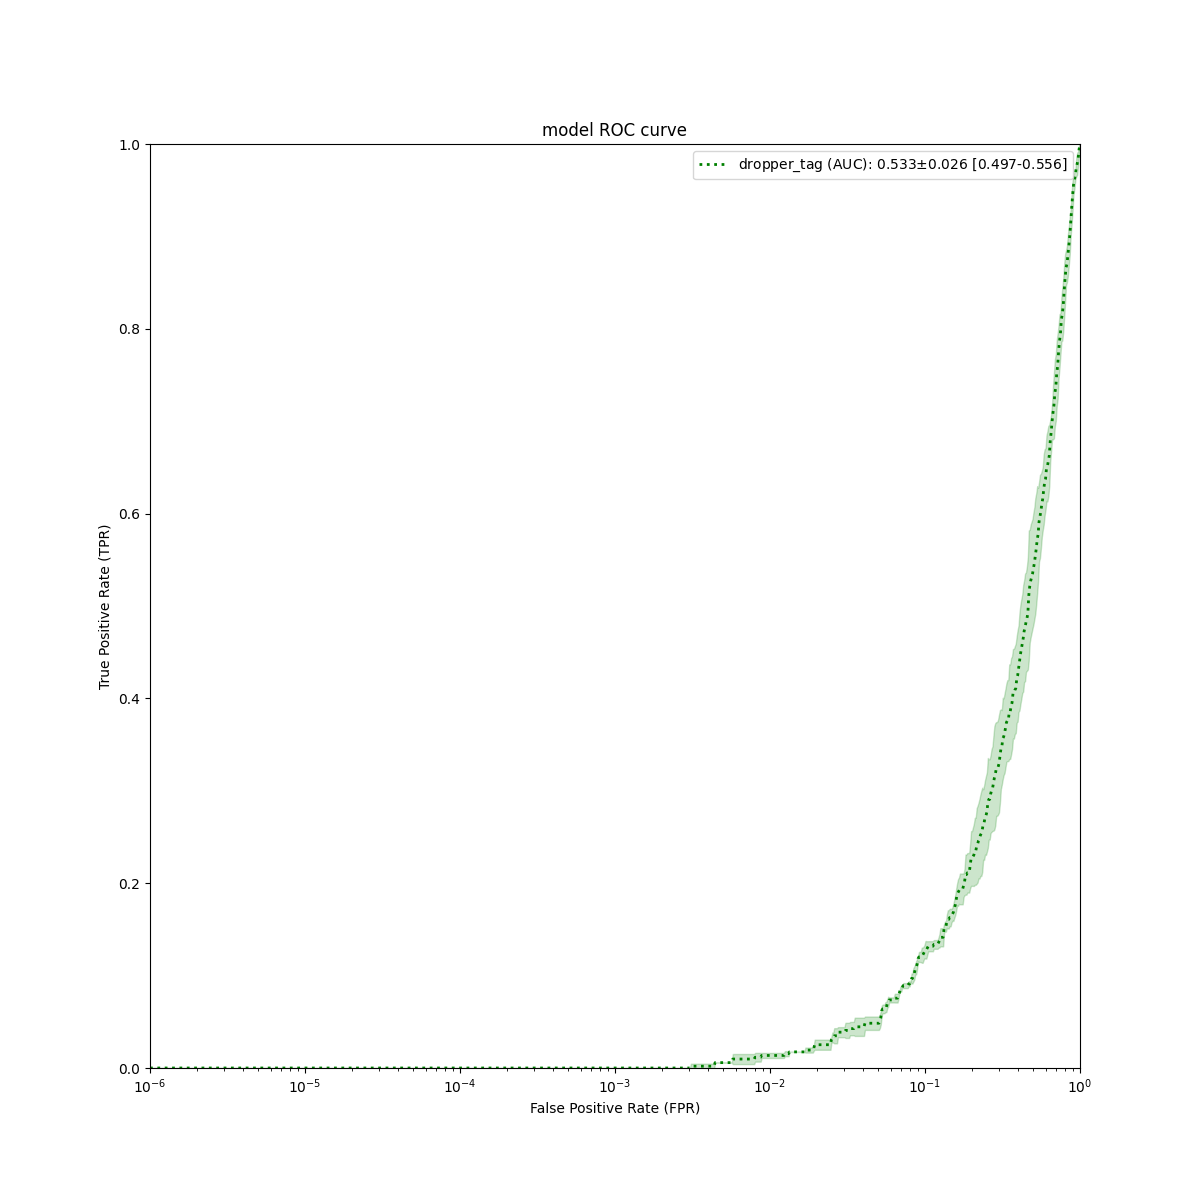
\includegraphics[width=0.6\textwidth]{./results/dropper_tag_roc_aloha.png}
        \vspace*{-0.2cm}
        \caption[Dropper Tag prediction task ALOHA ROC curve]{ROC curve and AUC statistics of \textBF{ALOHA} model for the \textbf{Dropper Tag}. The line represents the \textit{mean} TPR at a given FPR, while the shaded region represents the \textit{standard deviation}. Statistics were computed over \textBF{2} training runs, each with random parameter initialization.}
        \label{fig:dropperTagRocAloha}
    \end{figure}
}

\newcommand{\dropperTagRocProposedMethod}{
    \begin{figure}[H]
        \vspace*{-0.5cm}
        \centering
        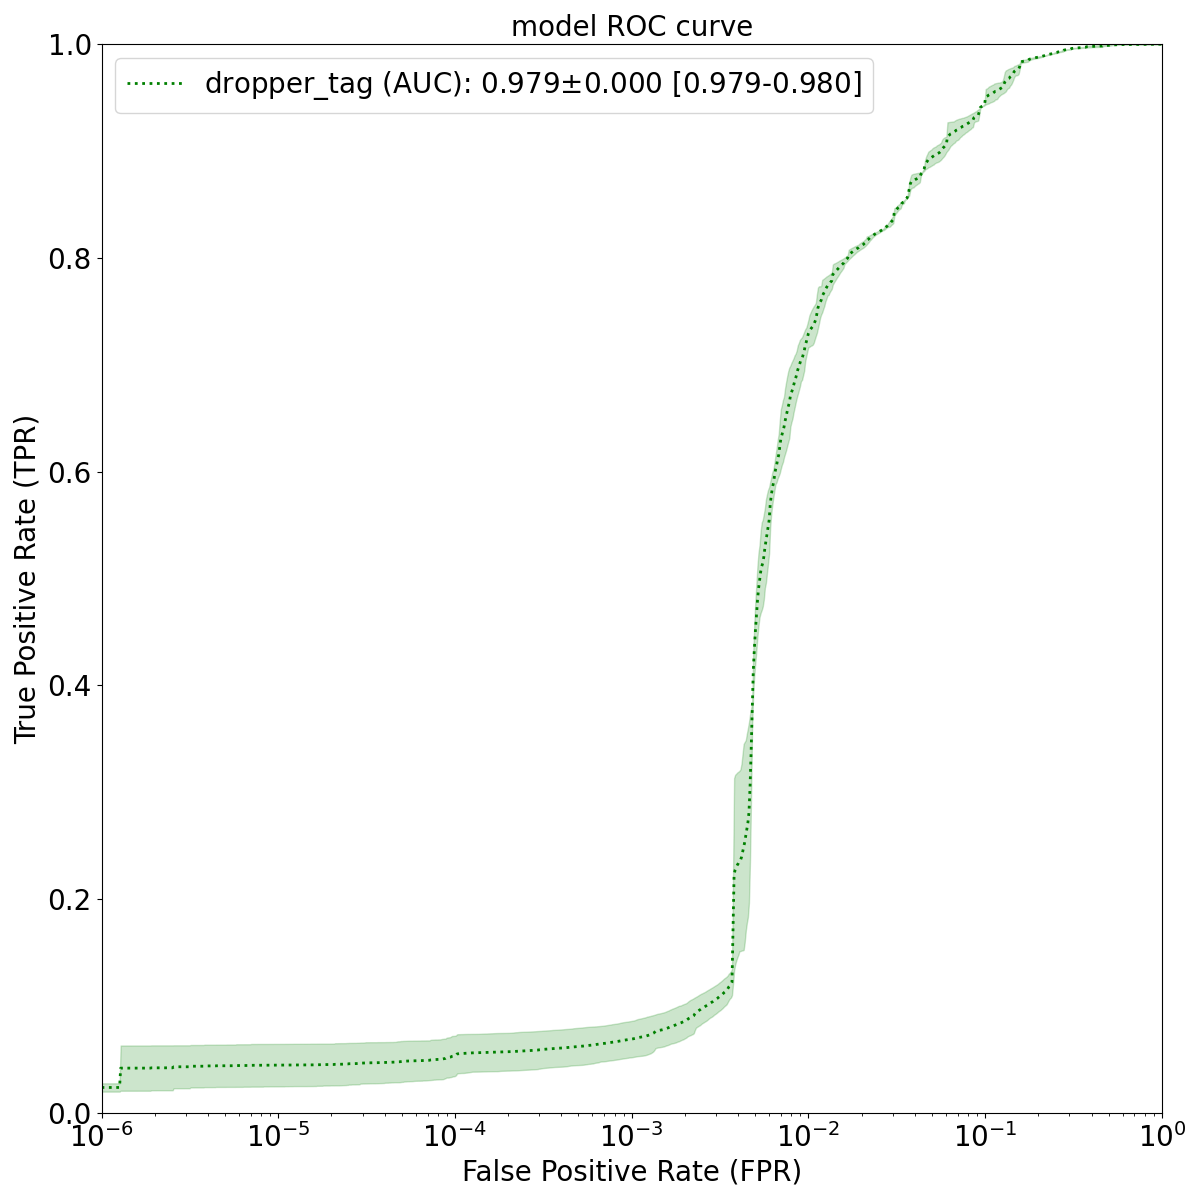
\includegraphics[width=0.6\textwidth]{./results/dropper_tag_roc_proposedModel.png}
        \vspace*{-0.2cm}
        \caption[Dropper Tag prediction task Proposed Model ROC curve]{ROC curve and AUC statistics of \textBF{Proposed Model} for the \textbf{Dropper Tag}. The line represents the \textit{mean} TPR at a given FPR, while the shaded region represents the \textit{standard deviation}. Statistics were computed over \textBF{2} training runs, each with random parameter initialization.}
        \label{fig:dropperTagRocProposedModel}
    \end{figure}
}
